\section{Introduction}
\label{sec:introduction}

Cyber-physical systems (CPS) are next generations of networked and
embedded systems, tightly coupled with computations and physical
elements to control physical phenomenon.
Control algorithms of CPS, therefore, are becoming more and more
complex, which makes CPS distinguished from traditional safety-critical
systems.
In CPS applications, the real-fast is as important as the real-time,
while only the real-time is a primary concern in safety-critical systems. 
This double-edge requirement of the real-time and the real-fast,
however, has posed a core challenge of CPS platforms.

\begin{figure}[tb]
 \centering
 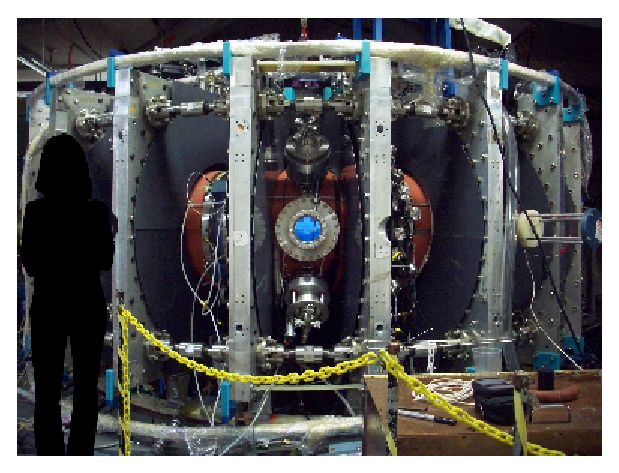
\includegraphics[width=0.8\hsize]{eps/tokamak.eps}
 \caption{The HBT-EP ``Tokamak'' at Columbia University.}
 \label{fig:tokamak}
\end{figure}

Plasma control for fusion is an applications of energy CPS, where
complex algorithms must be computed at a very high rate.
Figure~\ref{fig:tokamak} shows the HBT-EP Tokamak at Columbia
University~\cite{Maurer_PPCF11,Rath_FED12} that magnetically controls
the 3-D perturbed equilibrium state of the plasma~\cite{Boozer_PP99}.
It is required to process 96 inputs and 64 outputs of 16-bit data at a
sampling rate of a few microseconds.
An initial attempt of the Columbia team employed fast CPUs or FPGAs, but
even the simplified algorithm failed to run within 20$\mu$s.
An alternative approach was to parallelize the algorithm for the
graphics processing unit (GPU) using CUDA~\cite{CUDA}, the most
successful massively parallel computing technology.
However, the current system for GPU computing is not designed to
integrate sensor and actuator devices.
This is largely attributed to the fact that the GPU computing stack is
independent of I/O device drivers.
Since it may take tens of microseconds to transfer hundreds of bytes
between the CPU and the GPU, the current system does not allow plasma
control to use the GPU.
This is a signficant problem not only for plasma control but also for
many applications of CPS that utilize compute devices with I/O devices.

To the best of our knowledge, there is currently no generic support for
direct communication between the GPU and I/O devices, though a
specialized proprietary product for InfiniBand networks is
available~\cite{GPUDirect}.
There are also pinned memory allocation methods available from current
programming frameworks to reduce data-copy operations, but it is unclear
if they are best suited for real-time GPU applications. 
Although GPUs have been increasingly utilized in the domain of
CPS~\cite{Hirabayashi_REACTION12, Mangharam11, McNaughton_ICRA11,
Michel_IROS07}, and GPU resource management techniques have been
invented~\cite{Elliott_RTS12, Elliott_ECRTS12, Kato_RTAS11, Kato_RTSS11,
Kato_ATC11, Kato_ATC12, Liu_PACT12}, an integration of I/O processing
and GPUs remains an open problem.

In this paper, we present a zero-copy I/O processing scheme for GPU
applications.
This scheme incorporates functions and their application programming
interface (API) for I/O device drivers to directly transfer data to and
from GPU memory space, removing additional data-copy operations between
the CPU and the GPU.
We also investigate exisiting approaches, and compare them to the
presented zero-copy I/O processing scheme.
Our case study uses the Columbia University's Tokamak plasma control
system to evalaute a reduced sampling rate of plasma control.
In order to evaluate more generic properties of I/O processing schemes,
we further provide microbenchmarks, and discuss the pros and cons of each
scheme.
By clarifying GPU capabilities, we aim to not only improve the overall
performance but also broaden the scope of CPS that can benefit from the
use of GPU technology.


